\chapter{Tecnologías}
\label{sec:system}


En este capítulo se detallará la estructura, tecnologías y decisiones tomadas en el desarrollo del proyecto.


\section{Estructura final}

Las decisiones de las que se hablarán en este capítulo tienen como finalidad obtener la estructura final del sistema. Esta estructuración tiene como finalidad generar un sistema escalable tanto horizontalmente, es decir, que cada uno de los módulos puede ser redimensionado sin afectar al resto, p. ej. distribuyendo cada uno de los módulos en un servidor, y verticalmente, p. ej. aumentando los recursos de un servidor concreto para mejorar el rendimiento.

La estructura final y los detalles de las conexiones entre los diferentes subsistemas que se pretende conseguir se pueden ver en la \cref{fig:detailed_schema}.

\cfig{images/arquitectura/acatia-esquema-detallado.png}{Esquema detallado del sistema de streaming}{fig:detailed_schema}


\section{Arquitectura}
En el desarrollo de un proyecto de software es necesario definir una arquitectura que nos permita crear un sistema robusto y escalable.

En este proyecto se ha utilizado una arquitectura de tres capas [\cref{fig:high_level_arch_schema}] que se distribuye de la siguiente manera:

\begin{itemize}[noitemsep]
    \item \textbf{Capa de presentación}: Es la encargada de presentar y capturar la información del usuario.
    \item \textbf{Capa de negocio}: Es donde residen los programas que se ejecutan, recibe las peticiones del usuario.
    \item \textbf{Capa de datos}: Es donde residen los datos y es la encargada de acceder a los mismos.
\end{itemize}


\cfig{images/tech/arquitectura_capas.png}{Arquitectura de tres capas}{fig:high_level_arch_schema}


\section{Capa de Presentación}

En esta sección se comentará las diferentes tecnologías usadas para desarrollar las dos aplicaciones que conforman esta capa.


\subsection{Aplicación de captura de datos}
\label{sec:system:app_capture}

Esta aplicación permite capturar los datos del ratón en todo el escritorio del usuario y enviarlos al sistema de colas. Para el desarrollo de la aplicación se decidió utilizar \textit{Java} por las siguientes razones:

\begin{itemize}[noitemsep]
    \item \textbf{Multiplataforma:} Se puede ejecutar en la mayoría de sistemas operativos y dispositivos, con una única base de código.
    \item \textbf{Java Native Interface:} Permite ejecutar librerías nativas para interaccionar con elementos de bajo nivel.
\end{itemize}

La aplicación se ejecuta en segundo plano capturando los datos y enviándolos al servidor. Además, la aplicación cuenta con un menú contextual activar y desactivar el servicio de captura~[\cref{fig:desktop_app}].

\cfig[0.3\linewidth]{images/desktop-app/desktop_app.png}{Menú de la aplicación de escritorio.}{fig:desktop_app}

\subsection{Aplicación de administración}
\label{sec:system:web_admin}

Esta aplicación permite mostrar el estado del sistema en tiempo real. Para el desarrollo de la aplicación se decidió usar el framework \textit{Angular} por las siguientes razones:

\begin{itemize}[noitemsep]
    \item \textbf{Estructuración:} Proporciona un sistema por módulos que ayuda a organizar la aplicación separándolas por componentes.
    \item \textbf{Mantenimiento:} Permite modificar o reemplazar componentes con nuevas mejoras de una forma ágil.
\end{itemize}

Para las conexiones que se realizan contra el servidor se utilizan \textit{WebSockets} en vez de \textit{HTTP}, debido a las ventajas que ofrece en este tipo de sistemas:

\begin{itemize}[noitemsep]
    \item \textbf{Alto rendimiento:} Proporciona un canal de comunicación bidireccional, lo que nos permite enviar y recibir gran cantidad de datos de forma más eficiente.
    \item \textbf{Ahorro recursos:} Solo es necesario establecer una conexión y mantenerla abierta a la espera de recibir los datos. El establecimiento de la conexión tiene un coste más bajo que una conexión \textit{HTTP}.
\end{itemize}


Los mensajes que se obtienen por \textit{WebSockets}~\cite{ConsumeApache} se almacenan de manera local utilizando el patrón \textit{Redux} [\cref{fig:redux}]. Este patrón mantiene un objeto inmutable global en formato \textit{JSON} y solo es modificable mediante las acciones predefinidas. A pesar de que el uso de este patrón tiene un impacto negativo en el rendimiento, proporciona algunas ventajas a tener en cuenta:

\begin{itemize}[noitemsep]
    \item \textbf{Acceso global:} Es accesible desde cualquier punto de la aplicación. Esto permite crear componentes que pueden obtener los datos sin depender de otros.
    \item \textbf{Inmutable:} Solo se puede modificar con las acciones creadas por el desarrollador, dando un control exhaustivo sobre que modificaciones se pueden llevar a cabo.
    \item \textbf{Precarga:} El objeto creado permanece en el tiempo, haciendo que en visitas posteriores los datos se encuentren precargados y listos para mostrar.
\end{itemize}


\cfig{images/tech/acatia-redux.png}{Patrón Redux}{fig:redux}

Por defecto, \textit{JavaScript} utiliza un único hilo y este se utiliza para el procesamiento de los datos y dibujar de la interfaz. Esto implica que al procesar una gran cantidad de datos, el hilo y la interfaz de usuario quedan bloqueados durante ese tiempo. Por ello, se planteó el uso de \textit{WebWorker} que permite crear un hilo para ejecutar el procesamiento de los datos, dejando el hilo principal para la interfaz de usuario. Este planteamiento mejora el rendimiento y ofrece una experiencia fluida en la interfaz de usuario.


\subsubsection{Angular}
\label{sec:system:web_admin:angular}

Este framework sigue el patrón Modelo-Vista-Vista-Modelo [\cref{fig:MVVM}], el cual es una modificación del patrón Modelo-Vista-Controlador que se produce por el \textit{two-way-binding} que se da en \textit{Angular}.

\cfig[0.7\linewidth]{images/tech/acatia-MVC.png}{Patrón modelo-vista-vista-modelo}{fig:MVVM}


La aplicación desarrollada permite ver la información del sistema en tiempo real. La \cref{fig:generate_events} muestra la pantalla principal donde se puede ver una gráfica con los eventos que llegan al servidor a tiempo real.

\cfig{images/web/eventos_generados.png}{Ventana con la gráfica de eventos generados}{fig:generate_events}


En otra pantalla de la aplicación se listan los usuarios que hay en el sistema, pudiendo observar de un solo vistazo cual es el estado de cada uno de ellos y acceder al detalle del usuario [\cref{fig:user_stats}]. Esta ventana de detalle muestra una conjunto de gráficos con el ratio de autenticaciones satisfactorias y el tiempo de latencia de los eventos. Esta información ayuda al administrador del sistema a responder en tiempo real ante una incidencia.

\cfig{images/web/user_list.png}{Ventana de la lista de usuarios}{fig:user_list}
\cfig{images/web/user_stats.png}{Ventana de estadísticas del usuario}{fig:user_stats}

\section{Capa de Negocio}
La capa de lógica de negocio es la encargada de procesar los eventos y obtener las predicciones. Esta capa esta compuesta de un conjunto de tres servicios:

\begin{itemize}[noitemsep]
    \item \textbf{Sistema de gestión de colas}: Es el encargado de manejar los eventos y distribuirlos entre los diferentes servicios del sistema.
          El servidor encargado de manejar los eventos y distribuirlos entre los diferentes aplicativos finales.
    \item \textbf{Machine Learning}: Se el encarga de manejar todos los procesos relacionados con la Inteligencia Artificial, como la generación de modelos y la obtención de predicciones.
    \item \textbf{Orquestador}: Este servicio permite automatizar los procesos de generación de modelos y creación de máquinas.
\end{itemize}

El esquema general de este sistema se puede ver en la \cref{fig:medium_arch}, en él se observan las conexiones entre los diferentes servicios y capas, además se puede ver la composición de las máquinas de cada servicio.

\cfig{images/arquitectura/acatia-arquitectura_medio_nivel.png}{Esquema de la capa de negocio}{fig:medium_arch}


Esta estructuración se realizó pensando en la estabilidad del sistema, permitiéndonos aumentar el número de nodos de un servicio independientemente de otro.

\subsection{Docker}

Es una plataforma de virtualización a nivel de sistema operativo que nos permite crear una aplicación y empaquetarla junto con sus dependencias y librerías en un contenedor. Esta virtualización nos ofrece una serie de ventajas a la hora de crear y desplegar las aplicaciones:

\begin{itemize}[noitemsep]
    \item \textbf{Autocontenido:} El contenedor creado contiene todas las dependencias necesarias para la ejecución del programa, lo que implica que los servidores solo deben tener instalado \textit{Docker}.
    \item \textbf{Mayor consistencia:} Las pruebas se hacen dentro de un contenedor y el despliegue es el mismo. Esto implica que el entorno es idéntico en ambos casos.
    \item \textbf{Ligeras:} Las instancias creadas con \textit{Docker} son más ligeras que un sistema de virtualización tradicional.
    \item \textbf{Actualizaciones:} La actualización de los contenedores se realiza de forma sencilla, actualizando solo la versión de la imagen creada.
    \item \textbf{Aislamiento:} \textit{Docker} garantiza que cada contenedor se encuentre aislado por defecto, garantizando que tenga sus propios recursos.
\end{itemize}


\subsection{Sistemas de gestión de colas}
Este servicio se encarga de distribuir los mensajes entre los distintos aplicativos del sistema. Para ello se decidió utilizar el patrón publicación-suscripción [\cref{fig:pub_sub_schema}] que nos permite manejar una gran cantidad de datos en tiempo real.

\cfig{images/esquema_pub_sub.png}{Esquema Publicador/Suscriptor}{fig:pub_sub_schema}

En el mercado existen diferentes productos que implementan este patrón y permiten desplegar un servidor, de los que destacan:

\begin{itemize}[noitemsep]
    \item \textbf{RabbitMQ~\cite{AMQP, AMQP_IEEE}:} Es un proyecto de código abierto que implementa el estándar de mensajería \textit{AMQP} para casos de uso  de colas de baja latencia.
    \item \textbf{Kafka~\cite{kreps2011kafka}:} Es una plataforma de transmisión de eventos distribuida de código abierto y uno de los proyectos más activos de Apache.
\end{itemize}



\begin{table}[htbp!]
    \centering
    \begin{tabular}{ l  c c }
        \toprule
                           & \textbf{Kafka} & \textbf{RabbitMQ}                                                                                                      \\
        \midrule \midrule
        Rendimiento máximo & 605 MB/s       & 38 MB/s                                                                                                                \\ \midrule
        Latencia           & 5 ms           & 1 ms\tablefootnote{Las latencias de RabbitMQ se degradan significativamente a velocidades superiores a los 30 MB/s} \\ \bottomrule
    \end{tabular}
    \caption{\label{tab:queue_latency} Latencias y rendimiento de los distintos productos~\cite{nikhil_chandar_2020}}
\end{table}


De las opciones disponibles se optó por \textit{Kafka} por las siguientes razones:
\begin{itemize}[noitemsep]
    \item \textbf{Flujo de datos:} Nuestra aplicación genera 400 mensajes por usuario y segundo, ambas opciones deberían soportan bien este flujo de datos, pero \textit{Kafka} ofrece un mejor rendimiento.
    \item \textbf{Streams:} \textit{Kafka Streams} es una tecnología que nos permite procesar los datos realizando transformaciones y divisiones.
    \item \textbf{Consumidores:} Nuestra aplicación necesita que algunos datos sean consumidos por varios procesos y en este caso \textit{Kafka} nos permite hacerlo de forma nativa.
\end{itemize}


\subsection{Machine Learning}

Este proceso se encargará de toda la parte de Inteligencia Artificial que engloba los siguientes procesos:

\begin{itemize}[noitemsep]
    \item \textbf{Entrenamiento modelo:} Genera el modelo de Inteligencia Artificial de un usuario.
    \item \textbf{Transformación de datos:} Realiza la transformación de los datos en bruto.
    \item \textbf{Predicción:} Obtiene la predicción del modelo.
\end{itemize}


Para este sistema se utilizó el lenguaje de programación \textit{Python} debido a la versatilidad que ofrece en el análisis de datos y \textit{Java} para el proceso de transformación dada su compatibilidad con \textit{Kafka Streams}.

\subsection{Orquestador}

Este proceso se encarga de automatizar el proceso de creación de modelos y máquinas de predicción  haciendo uso de las \textit{API} de \textit{Docker} y \textit{Kafka}.
La \cref{fig:orquestation_schema} muestra la estructura y en ella podemos como el proceso de orquestación  obtiene los datos de las API y se encarga de realizar las llamadas correspondientes a los subprocesos de generación de modelos y creación de la máquina de predicción:

\begin{itemize}[noitemsep]
    \item \textbf{Generación de modelos:} Accede a la base de datos para obtener los eventos del usuario, generar el modelo correspondiente a ese usuario y guardar ese modelo en disco.
    \item \textbf{Máquina de predicción:} Configura una nueva máquina basándose en los parámetros del usuario y modelo, desplegándola automáticamente sin interacción por parte de un administrador.
\end{itemize}

\cfig{images/orquestation/orquestador_schema.png}{Workflow del sistema de orquestación}{fig:orquestation_schema}

Este sistema ejecuta un proceso que mapea las máquinas y modelos existentes con los usuarios, obteniendo en el proceso la relación de usuarios que no disponen de modelos o máquinas de predicción. El flujo de trabajo de este proceso se puede ver en detalle en las \cref{fig:orquestation_worflow,fig:workflow_model}, donde se puede observar la lógica de la creación de un modelo y las diferentes comprobaciones que se llevan a cabo para que dicho modelo tenga una calidad aceptable.


\begin{figure}[htbp!]
    \centering
    \begin{minipage}{.49\textwidth}
        \centering
        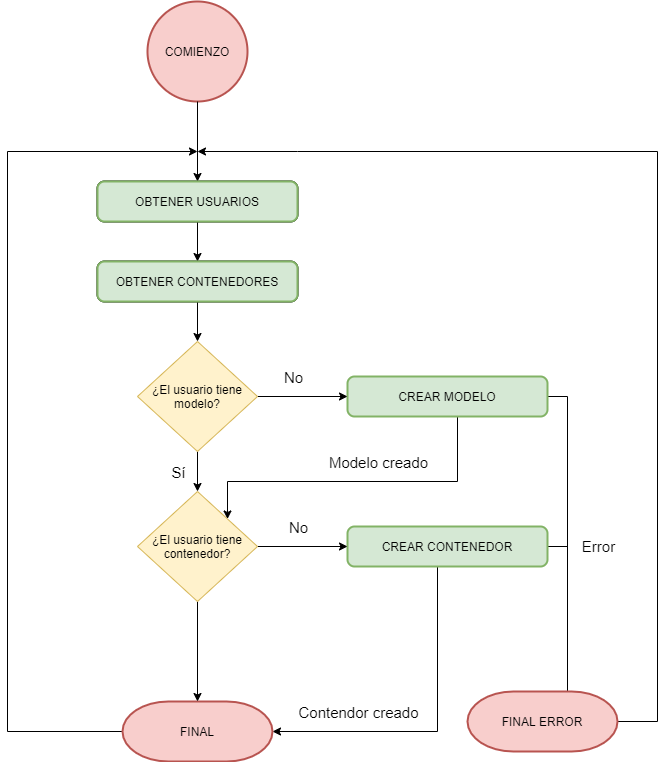
\includegraphics[width=\linewidth,keepaspectratio]{images/orquestation/workflow.png}
        \caption{Flujo del sistema de orquestación}
        \label{fig:orquestation_worflow}
    \end{minipage}
    \begin{minipage}{.49\textwidth}
        \centering
        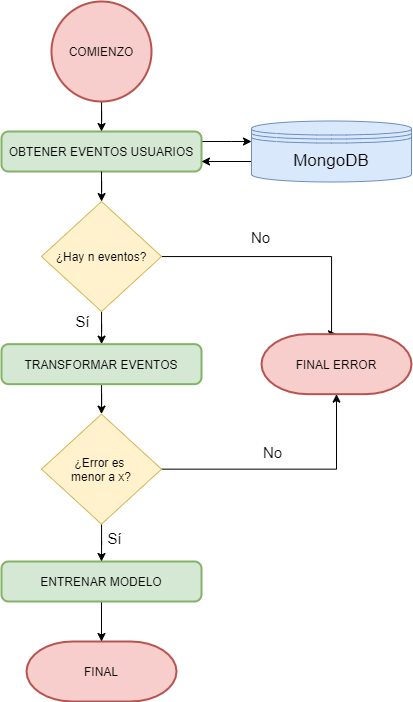
\includegraphics[width=\linewidth,keepaspectratio]{images/orquestation/workflow_model.png}
        \caption{Flujo de creación de modelos}
        \label{fig:workflow_model}
    \end{minipage}

\end{figure}

\subsection{Capa de Datos}

Esta capa se utilizará para almacenar los datos de entrada de manera persistente, para realizar operaciones en el futuro como creación o actualización de nuevos modelos, búsqueda de nuevas características o técnicas de inteligencia artificial.

Como base de datos se ha decidido usar \textit{MongoDB}, una base de datos NoSQL. Los motivos por los que se ha elegido este tipo de base de datos frente a otras (relacional) son:

\begin{itemize}[noitemsep]
    \item \textbf{Velocidad:} Una de las principales ventajas de esta base de datos es la prioridad en manejar lecturas, y en este caso es perfecto para nuestro sistema, debido a que la mayor parte de accesos serán de lectura.
    \item \textbf{Volumen:} La aplicación de captura genera una gran cantidad de datos y por lo tanto, necesitamos una base de datos que funcione en sistemas de \textit{Big Data}.
    \item \textbf{Variabilidad:} La aplicación manejará datos, que pueden no ser consistentes e incluso algunos de ellos pueden modificarse con el tiempo. Este tipo de base de datos no necesitan un esquema para trabajar por lo que las hace ideales para este tipo de casos.
\end{itemize}

\subsubsection{ReplicaSet}

Un \textit{ReplicaSet} en \textit{MongoDB}~[\cref{fig:replica_set}] es un grupo de instancias que mantienen el mismo conjunto de datos. Este sistema permite tener una alta disponibilidad y redundancia de datos.

En el proyecto se crearán tres instancias de \textit{MongoDB} donde la aplicación se conectará a la primaria y las otras instancias se sincronizarán con ella. Una de las ventajas que presenta este sistema es que permite trabajar de manera distribuida, de modo que si un nodo se cae el resto puede asumir el trabajo y el sistema no se ve afectado.

\cfig{images/arquitectura/replicaset.jpg}{Estructura replicaSet~\cite{mongoReplication}}{fig:replica_set}


